bf{NFT Use Cases}

bf{Art}

The recent surge of interest in NFT's during early 2021 has largely been
driven by digital art NFT's, despite the origins of digital art NFT's
started much earlier in 2014. New York artist
\href{https://www.mccoyspace.com/project/125/}{Kevin McCoy's
\emph{Quantum}} is widely recognised as the first piece of art created
as an NFT. However it was during early 2021 that art NFT's started to
gain significant attention; by the end of 2021, nearly
\href{https://www.paymentscardsandmobile.com/state-of-the-blockchain-nfts-explode-onto-scene-in-2021/}{£31b
had been spent} on NFT purchases, a considerable and exponential growth
given
\href{https://raritysniper.com/news/nfts-exploded-in-2021-with-25-billion-in-sales/}{2020
sales of asciitilde£71m}

High profile digital artists such as \emph{Beeple} whose
\href{https://www.forbes.com/sites/abrambrown/2021/03/11/beeple-art-sells-for-693-million-becoming-most-expensive-nft-ever/?sh=3f237d1c2448}{recent
recording break sale} of his NFT \emph{``The first 5000 days''} (Figure \ref{fig:first5000days}) at Christies (a long established British auction house,
specialising in high profile precious work of art) for £52.9m helped
bring NFT's into the public spotlight and wider give them global
attention.

\begin{figure*}[ht]\centering % Using \begin{figure*} makes the figure take up the entire width of the page
	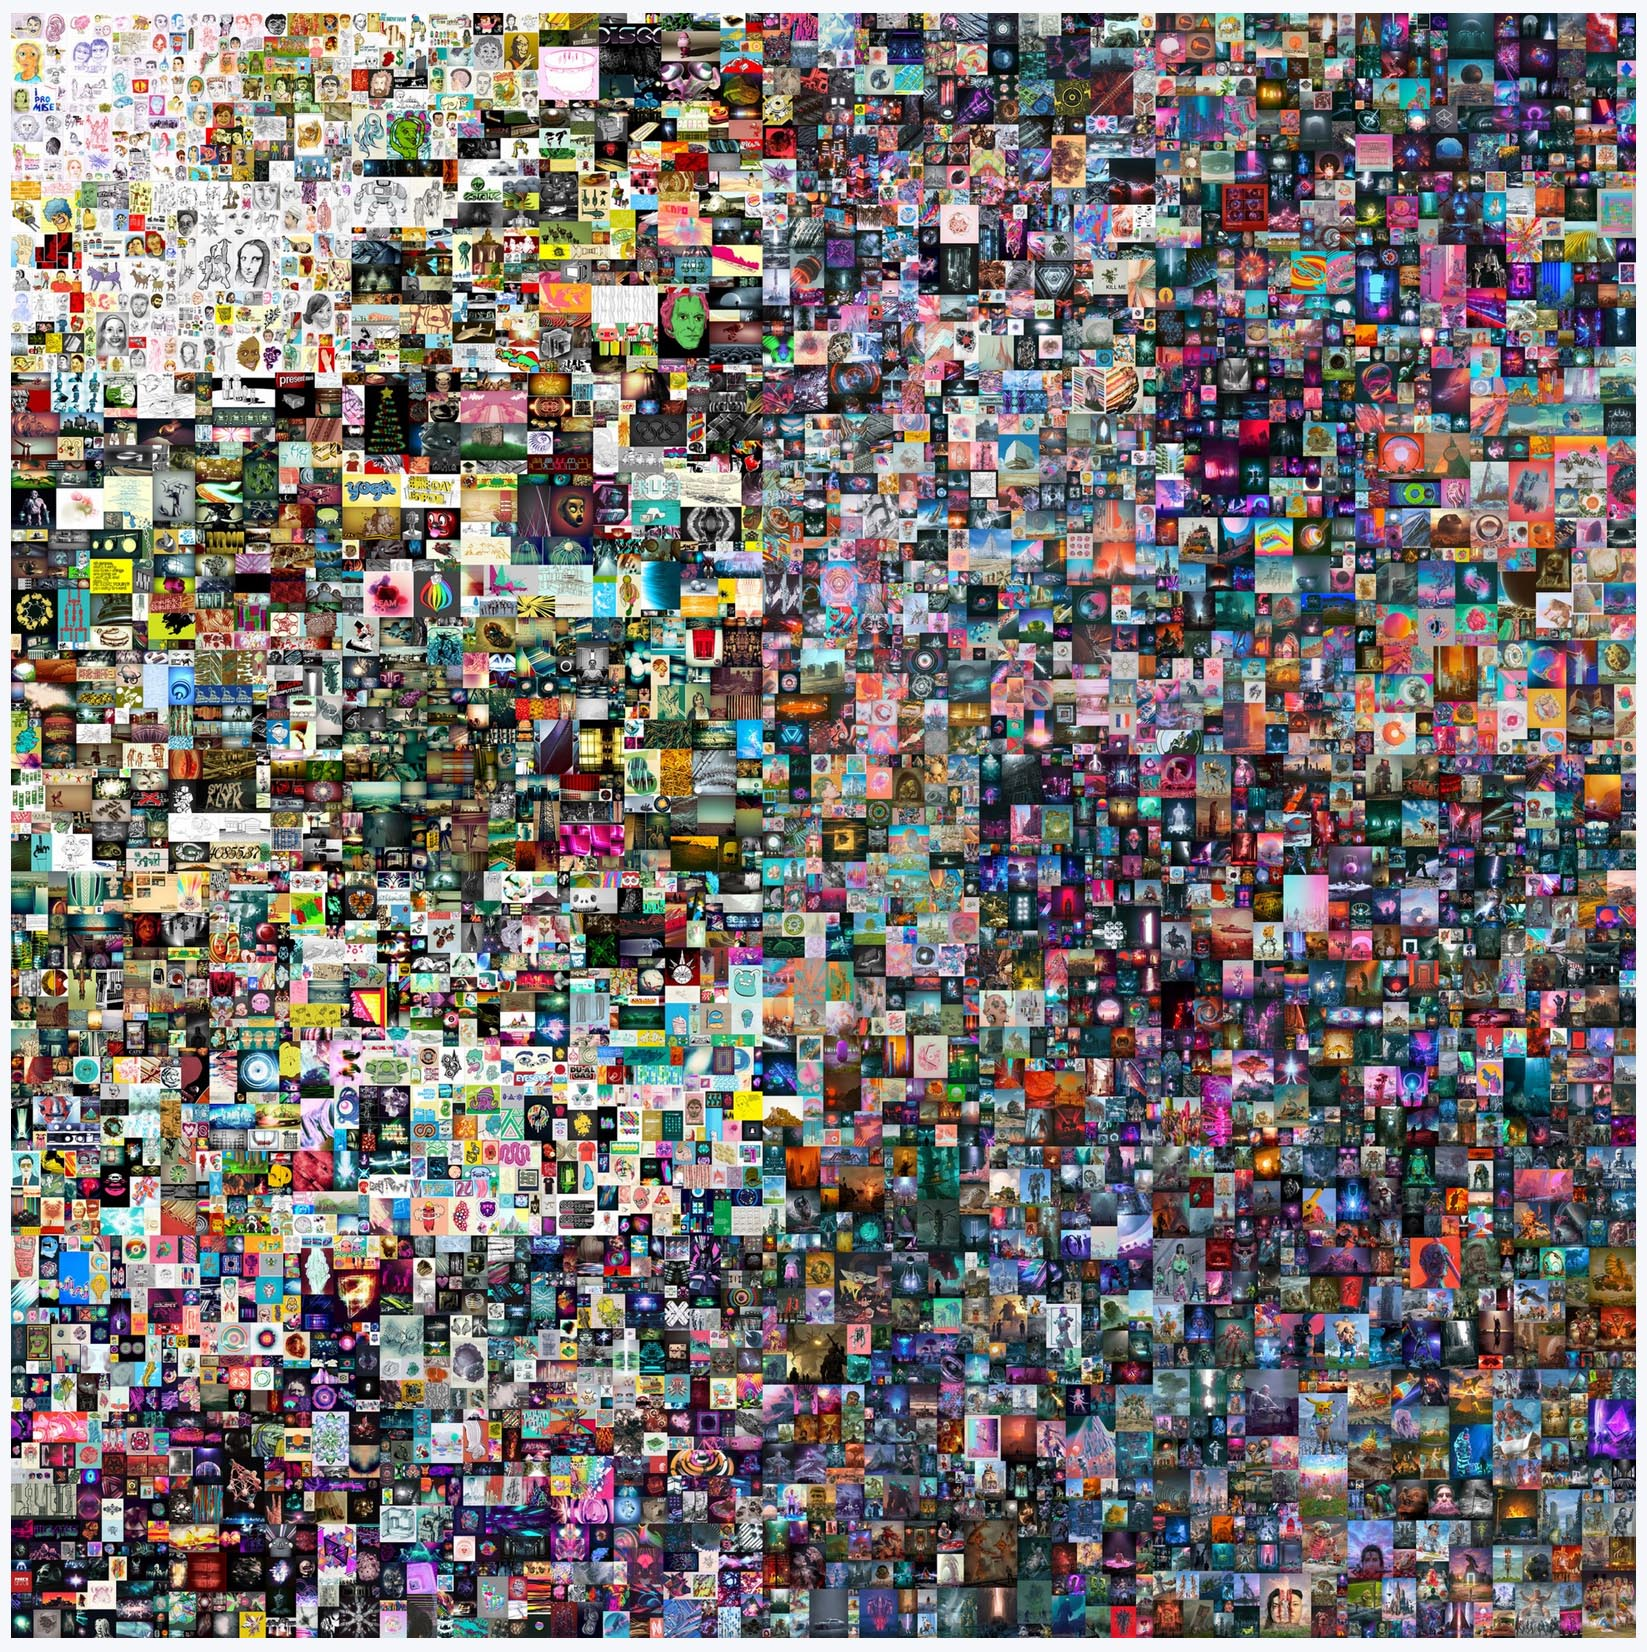
\includegraphics{first5000days}
	\caption{Beeple: First 5000 days, \href{https://onlineonly.christies.com/s/beeple-first-5000-days/lots/2020}{taken from the Christies website, assumed fair use}.}
	\label{fig:first5000days}
\end{figure*}

Art as NFT's offer the following advantages:

\begin{enumerate}
\def\labelenumi{\arabic{enumi}.}
\item
  \textbf{Immutable Nominal Authenticity:} Art fraud such as false
  representation, forgeries, plagiarism have been a reoccurring blight
  since art has existed; artists and works of art have been open to
  abuse by forgers, black market profiteers and even fellow artists
  laying claim to works of art of others. Unless a work of art is sold,
  exhibited or listed, documenting when and who created it, the
  \emph{nominal authenticity,} which Dutton states as the
  \emph{``correct identification of the origins, authorship, or
  provenance of an object''} \cite{dutton2003authenticity} can be increasingly mutable over a period
  of time, dependent on a multitude of factors, including; the artists
  existing profile, how widely and where the work of art is exhibited,
  if the work of art is commissioned by a patron, if it's sold, and
  profile of the buyer/collector. At its most basic level, once a work
  of art is `minted' as an NFT (publishing the art work as a unique
  token on the blockchain) this functions as an immutable publicly
  accessible proof of ownership and by extension proof of creation. The
  act of minting is not purely limited to digital art; all an artist
  requires is a digital representation of any physical art (sculpture,
  physical painting, installation etc..) which can be used as a proxy
  allowing artists to record the date of creation/origin of a physical
  piece of art on the blockchain, a buyer purchasing the NFT can be
  provided the actual physical artwork as part of the NFT. Nominal
  authenticity becomes secure and immutable.

  \begin{enumerate}
  \def\labelenumii{\alph{enumii}.}
  \item
    \textbf{Secure Digital Provenance}:
    \href{https://en.wikipedia.org/wiki/Provenance}{Provenance} (or the
    chain of custody) is an important aspect in works of art, antiques
    and antiquities. Provenance not only helps assign work to an artist
    but also documents ownership history. Digital provenance, an
    inherent feature of NFT's means provenance now no longer becomes
    what has historically sometime been a contentious detective's game
    at the best of times; one that is open to fraud, misinterpretation
    and entirely reliant on good record keeping.
  \end{enumerate}
\end{enumerate}

Since provenance can contribute to the value of a piece of art
(benefiting both the creator and collector) the use of the blockchain as
an open, secure ledger is a far more trustworthy system than traditional
methods of artistic provenance that were cobbled together; often
consisting of a mix of physical and digital documents spanning private
\& public sale receipts, art/museum gallery exhibitions and private
record keeping). Digital provenance provided when an artist `mints' a
piece of art into an NFT allows artists and collectors to record a
secure, permanent unalterable history of transactions for a specific
piece of art, providing future collector complete trust in the origin
and custody of a piece of art.

\begin{enumerate}
\def\labelenumi{\alph{enumi}.}
\setcounter{enumi}{1}
\item
  \textbf{Decentralised automated royalty payments}: Traditionally if a
  piece of art is sold, the first sale may (but not always) benefit the
  artist financially, however secondary and any subsequent sales would
  only ever financially benefit the buyer/collector; the original artist
  would rarely benefit. However If a work of art is minted into an NFT,
  royalty payments can be predetermined and automated in perpetuity
  directly by the use of a `smart contract'. Smart contracts are small,
  automated scripts/programs that run automatically and independently of
  a buyer/seller; pre-determined conditions are set by the buyer; these
  trigger when certain conditions are met i.e

  \begin{enumerate}
  \def\labelenumii{\roman{enumii}.}
  \item
    \emph{On sale transfer 20\% of total sale amount into digital wallet
    of the creator.}
  \item
    \emph{On sale transfer 80\% of total sale amount into digital wallet
    of the seller.}
  \end{enumerate}
\end{enumerate}

Once the royalty payment rate is set by the artist/creator, future
royalties of all sales can be paid directly to the artist/creator
account (via a digital wallet) without the need of a third party
(traditionally a gallery/agent etc..).

Smart contract driven NFT's means that even if piece of art is resold 5,
10 or even a 100,000 times moving through 5, 10 or even a 100,000
different collectors; a pre-determined royalty payment rate set by the
creator would still guarantee the artist/creator is paid directly from
each and every future sale.

Historically provenance for works of art may span across generations,
for instance Gabriël Metsu's oil on canvas painting \emph{The Lace
Maker's} provenance, first recorded in 1722, now spans 300 years of
ownership, including from a British Baron in the 19superscript{th}
century to an American philanthropist in the 20superscript{th}
century.) Metsu died young at the age of 38, leaving a widow; neither
his/her relatives/descendants benefit from his original work, 300 years
later this would be near impossible to facilitate with traditional
systems, as even legal contracts are open and prone to the ravages of
time.

NFT smart contracts hold an incredibly potential; an artists descendants
financially benefiting directly from the resale of a piece of work long
after the artist/museum's/gallery or even state have turned to dust as
long as the original creator's digital wallet is accessible, \emph{the
blockhain becomes an everlasting digital patron} ensuring

bf{Computer \& Video Games}

Computer \& Video games are a huge global business, exponential global
growth over the last 30 years has seen this grow to a point where it has
eclipsed both the
\href{https://www.businessinsider.com/video-game-industry-revenues-exceed-sports-and-film-combined-idc-2020-12?r=US\&IR=T}{global
movie and North American sports industries} combined.

A global industry with revenues over £120b,
\href{https://www.wepc.com/news/video-game-statistics/}{with
asciitilde half the people on the planet} playing some form of
games in 2021.

As the games industry has evolved and matured over the last 40 years,
secondary markets have emerged, most notably the `second hand' games
resale market. The rise of `retro' gaming, has demonstrated the second
hand market is a lucrative one for private resellers, an unopened copy
of Super Mario Bros for the Nintendo Entertainment System
\href{https://www.nytimes.com/2021/08/06/business/super-mario-bros-sale-record.html}{recently
selling for £1.5M} to the extent the market has seen
\href{https://www.businessinsider.com/retro-gaming-market-being-overtaken-by-speculators-2021-9?r=US\&IR=T}{speculators
looking to cash in} on the huge global interest in retro/second hand
games

Despite publishers and developers increasingly moving to non-physical
digital only' games, the demand for used games remains incredibly high.

Whilst some retailers have adapted their business models to include
reselling of retro/second hand games, the vast majority of
publisher/developers/retailers aren't able to directly benefit from the
emerging retro/second hand games market. The potential of \emph{video
games as NFT's} presents a huge opportunity for publishers, developers
and players alike, offering the following advantages:

\begin{enumerate}
\def\labelenumi{\alph{enumi}.}
\item
  \textbf{Royalty Sales on Pre-owned Games} ; A predetermined proportion
  of any resale of a used game can automated in perpetuity via smart
  contracts; once these are set by the publisher, future royalties of
  all sales can be paid directly to the publishers/developers wallets (a
  digital account) without the need of a third party (traditionally a
  retail entity). Traditionally only the initial first sale of a game
  would financially benefit the publisher/developer/retailer, secondary
  and subsequent sales would only ever financially benefit the
  purchaser, with many developers/publishers arguing this is hurting the
  wider industry through the loss of significant income generated by the
  secondary and subsequent sales, sometimes over the course of decades.
  However the use of NFT's smart contracts means that if a game is
  sold/resold through 10,000 collectors; a pre-determined royalty
  payment rate set by the publisher would still guarantee the publisher
  (and or developer/retailer) takes a proportion of any future sales.
\item
  \textbf{Monetisation of User Generated Content:} Games as a NFT's
  offer ability to monetise UGC: User generated content.
\end{enumerate}

Video games such as
\href{https://www.businessofapps.com/data/pokemon-go-statistics/}{Nintendo's
\emph{Pokemon Go}} \emph{(166 million players)},
\href{https://techacake.com/destiny-2-player-count/\#:~:text=The\%20total\%20player\%20base\%20of,to\%20be\%2038\%20million\%20players.\&text=According\%20to\%20the\%20source\%2C\%20the,in\%20terms\%20of\%20player\%20population.}{Bungie's
\emph{Destiny 2}} \emph{(38 million players)} or
\href{https://fictionhorizon.com/how-many-people-play-genshin-impact/\#:~:text=Genshin\%20Impact\%20had\%20approximately\%209,million\%20users\%20in\%20June\%202021.}{miHoYo's
Genshin Impact} (\emph{9 million players} ) all have large, established
and significant player bases. What is noteworthy, the games are designed
to encourage players may spend hundreds, or in some cases thousands of
hours on one game alone; according to
\href{https://destinytracker.com/destiny/leaderboards/all/minutesplayedtotal?grouped=true\&page=1}{Destinytracker.com},
the top players have amassed total play times over 20,000 hours, close
to 1,000 days or asciitilde{} 3 years, which is incredible feat
given Destiny 2 only launched 5 years ago in 2017.

Destiny/Pokemon Go and Genshin Impact revolve around a central key game
mechanic; players investing significant amounts of time collecting in
game digital assets; characters/weapons/items, often classed as `rare'
or `exotic' or `5 Star'. These collectibles usually found by a
combination of the accrual of in-game time, completing quests,
purchasing additional in-game items/boosters, and luck (`RNG'). Players
are often encouraged to share their collections of rare
characters/weapons/ objects through in-game achievements, triumphs,
scores acting as a mark of distinction/status symbol.

Traditionally there has been nothing that went beyond sharing the
\emph{digital badge} (i.e triumph/achievement/accomplishment) on a on
social media/gamer's platform profile. However NFT's offer the ideal
system for developers/publishers and even players to monetise user
generated/customised data (such as a players unique save game data),
simultaneously allowing:

a) creation of an additional monetised ecosystem to meet player demands
i.e. some players who are willing to monetise and `sell' their invested
time in a particular product/service to other players with little time
but willing to pay other players for `grinding' (progressing laborious
in game tasks) and a more advanced in-game progression point.

The potential to provide publishers/developers with an additional
long-term income stream, providing a better ROI on computer \& video
game development, which in many instances can cost hundreds of millions
in development costs spanning 5/10 years, is undeniable.

\begin{enumerate}
\def\labelenumi{\alph{enumi}.}
\setcounter{enumi}{2}
\item
  Play to earn revenue models.
\item
  Monetizing In game collectibles: customisable in game assets (vanity
  items such as cosmetic character skins/clothing or collectible items
  that offer player advantages(new weapons/vehicles/mods etc,..)
\end{enumerate}

bf{Figure 1.x:} Typical Smart Contract Structure:
https://www.jigsawllc.com/2021/03/25/nfts-creativity-innovation/
